\documentclass{article}
\usepackage{authblk}
\usepackage{blindtext}
\usepackage{listings}
\usepackage{color}
\usepackage{amsmath}
\usepackage{amsthm}
\usepackage{graphicx}
\usepackage{amsmath,amssymb,amsthm}
\newcommand{\limp}{\Rightarrow}
\newcommand{\WP}[2]{\mathit{WP}(#1,#2)}
\newcommand{\SP}[2]{\mathit{SP}(#1,#2)}
\newcommand{\havoc}{\mathit{havoc}}
\newcommand{\guard}{\mathit{guard}}
\definecolor{codegreen}{rgb}{0,0.6,0}
\definecolor{codegray}{rgb}{0.5,0.5,0.5}
\definecolor{codepurple}{rgb}{0.58,0,0.82}
\definecolor{backcolour}{rgb}{0.95,0.95,0.92} 
\lstdefinestyle{mystyle}{
    backgroundcolor=\color{backcolour},   
    commentstyle=\color{codegreen},
    keywordstyle=\color{magenta},
    numberstyle=\tiny\color{codegray},
    stringstyle=\color{codepurple},
    basicstyle=\footnotesize,
    breakatwhitespace=false,         
    breaklines=true,                 
    captionpos=b,                    
    keepspaces=true,                 
    numbers=left,                    
    numbersep=5pt,                  
    showspaces=false,                
    showstringspaces=false,
    showtabs=false,                  
    tabsize=2
}
\newtheorem{mydef}{Definition}
\newtheorem{theorem}{Theorem}
\newtheorem{lemma}{Lemma}

\lstset{style=mystyle}
\usepackage[utf8]{inputenc}
\title{Fault Localization \& Relevance Analysis \\ }
\author{Numair Mansur, Christian Schilling, Matthias Heizmann}
\affil{University of Freiburg, Germany}
\begin{document}

\maketitle
\begin{mydef}[Execution]\label{mydef:execution_definition}
Let $\pi$ be an error trace of length $n$. An execution of $\pi$ is a sequence of states $s_0, s_1...s_n$ such that $s_i, s_{i+1} \models T$, where $T$ is the transition formula of $\pi[i]$. \\
Let $\epsilon$ represent the set of all possible executions of the error trace.
\end{mydef}

\begin{mydef}[Blocking Execution]\label{mydef:blockingexecution_definition}
An execution of a trace $\pi$ of size $n$ is called a blocking execution if there exists a sequence of states $s_0, s_1...s_j$ where $i<j \leq n$ such that $s_i, s_{i+1} \models T[i]$, where $T[i]$ is the transition formula of $\pi[i]$ and there exits an assume statement in the trace $\pi$ at position $j$ such that $s_{j} \not \limp guard(\pi[j])$.
\end{mydef}

\begin{mydef}[Relevancy of an assignment statement]\label{mydef:relevancy_definition}
Let $\beta$ represent the set of all blocking executions of a trace $\pi$. Let there be an assignment statement of the form $x:=t$ at position $i$. Let $\pi'$ represent the trace that we get after replacing $\pi[i]$ with a havoc statement of the form $havoc(x)$ and let $\beta'$ represent the set of all blocking executions for $\pi'$.\\
We say that the assignment statement $\pi[i]$ is relevant if the trace after the replacement has strictly more blocked executions than the trace before the replacement, i.e if $\beta \subsetneq \beta'$. 
\end{mydef}

\begin{lemma}[]\label{lemma:rel_bw_assignment_and_havoc}
For a predicate $Q$ and an assignment statement of the form $x:=t$ where $x$ is a variable and $t$ is an expression, we have:
$$WP(Q; havoc(x)) \subseteq WP(Q; x:=t)$$
\end{lemma}

\newpage

\begin{theorem}[Relevancy of an assignment statement]\label{mydef:relevancytheorem}
Let $\pi$ be an error trace of length $n$ and $\pi[i]$ be an assignment statement at position $i$ having the form $x:=t$, where $x$ is a variable and $t$ is an expression. Let $P$ and $Q$ be two predicates where $P = \neg WP(False; \pi[i,n]) \cap SP(True; \pi[1, i-1])$ and $Q =  \neg WP(False; \pi[i+1,n])$. The statement $\pi[i]$ is relevant iff:
 $$P \not \limp WP(Q,havoc(x))$$
\end{theorem}

\begin{proof}
Let $\pi'$ be the trace where the assignment statement $\pi[i]$ is replaced by a havoc statement. \\
"$\Rightarrow$" \\
If the assignment statement $\pi[i]$ is relevant then:
$$P \not \limp WP(Q,havoc(x))$$
Note that here we can also write $P$ as $WP(Q; x:=t) \cap SP(True; \pi[1, i-1])$.\\
Let $Q' := SP(P; havoc(x))$ and $P' := WP(Q;havoc(x)) \cap SP(True; \pi[1, i-1])$. \\
Since from lemma one, we know that 
$$WP(Q; havoc(x)) \subseteq WP(Q; x:=t)$$
and also,
$$WP(Q; havoc(x)) \cap SP(True; \pi[1, i-1])  \subseteq WP(Q; x:=t) \cap SP(True; \pi[1, i-1])$$
therefore:
$$P' \subseteq P$$
For simplicity in the proof, lets ignore the term $SP(True; \pi[1, i-1])$ from $P$ and $P'$. We simplify $P$ and $P'$ to be $WP(Q; x:=t)$ and $WP(Q; havoc(x))$ respectively. \\
\\
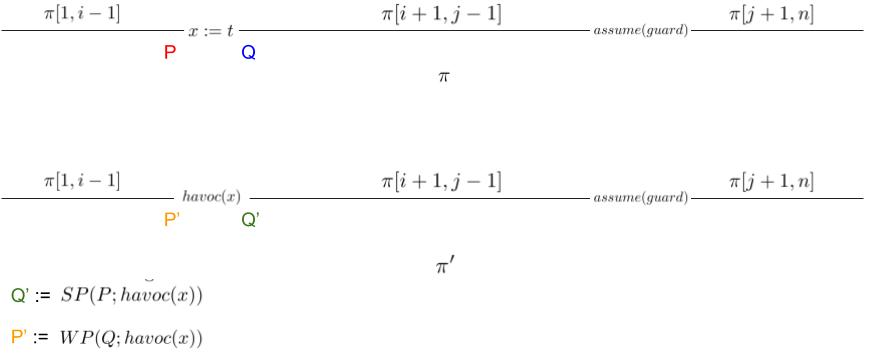
\includegraphics[width=\linewidth]{traces.jpg}\\
Relevancy of $x:=t$ implies that replacing it with $havoc(x)$ gives us strictly more blocking executions then before. Therefore
$$Q \subsetneq Q'$$
\newpage
Lets look at the following diagram to help us see the states a little better and come to the following conculsions:\\
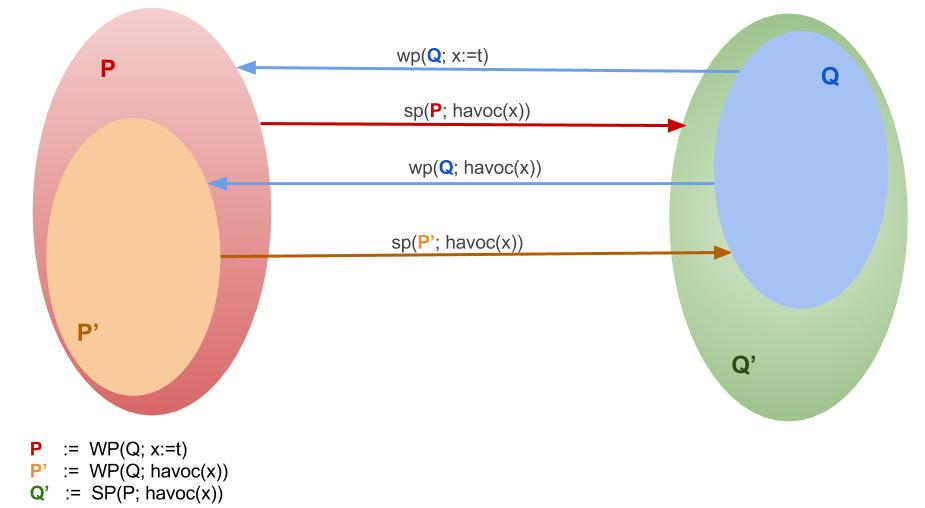
\includegraphics[width=\linewidth]{states.jpg}\\
$$SP(P; havoc(x)) = Q'$$
$$SP(P'; havoc(x)) = Q$$
and we know that $Q \subsetneq Q'$. This means that $\exists S \in P \setminus P'$, such that there is a transition from $S$ to $Q'$ if we execute $havoc(x)$. The existence of the state $S$ means:
$$P \not \limp P'$$
or
$$P \not \limp WP(Q; havoc(x))$$
\end{proof}
\end{document}